\section{Additional Efficiency Evaluation}
\label{app:efficiency}

Figure~\ref{fig:app-bs} reports the decode-step throughput on the B200 at context lengths from 1K to 8K, complementing the 4K results in Figure~\ref{fig:eval-e2e}.
Each bar stacks the FP32 throughput (lighter shade) and the gain of \method{} (darker shade).
For models that pair linear attention with dense full attention, the gain shrinks slightly as the context grows, since the full attention layers take a growing share of each step.
It remains substantial at 8K, where \method{} still accelerates Kimi-Linear-48B-A3B by 1.18$\times$ at batch size 512.
Recent models increasingly combine linear attention with sparse attention rather than full attention, which keeps the attention cost nearly constant as the context grows.
Figure~\ref{fig:app-long} evaluates two such models, GLM-5.3-Flash and Qwen3.8-Flash, up to 128K and 96K at batch size 256.
\method{} accelerates them by 1.25$\times$ and 1.23$\times$ at 4K and still by 1.23$\times$ and 1.20$\times$ at the longest context.
We therefore expect \method{} to perform equally well at very long contexts on upcoming hybrid models.

\begin{figure}[h]
    \centering
    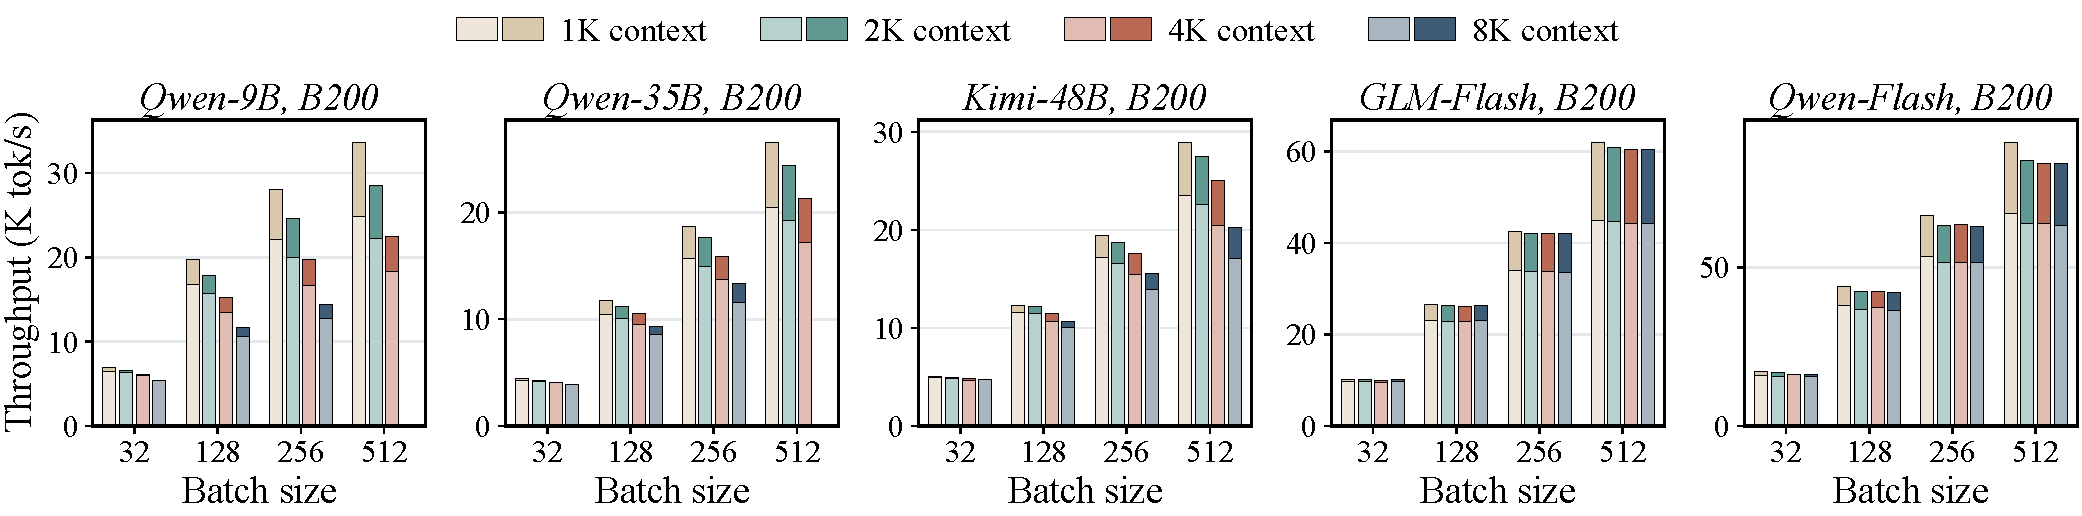
\includegraphics[width=\linewidth]{figures/app_decode_bs.pdf}
    \caption{Decode-step throughput in vLLM on the B200 at context lengths 1K--8K. Each bar stacks the FP32 throughput (lighter) and the gain of \method{} (darker).}
    \label{fig:app-bs}
\end{figure}

\begin{figure}[h]
    \centering
    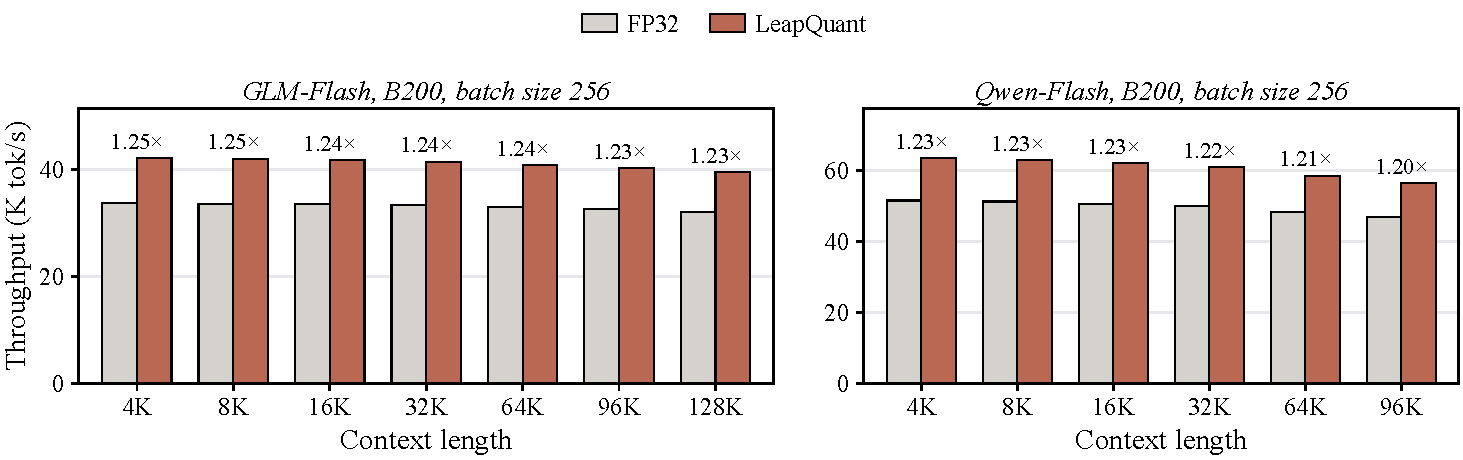
\includegraphics[width=0.85\linewidth]{figures/app_decode_long.pdf}
    \caption{Decode-step throughput of the two sparse-attention models on the B200 at batch size 256 and long contexts.}
    \label{fig:app-long}
\end{figure}
